\chapter{Quanto uma PTA pequena aprende: experimentos sintéticos}
\label{cap:simulacoes}

Os capítulos anteriores mostraram que as assinaturas massivas estão
concentradas nos primeiros canais de frequência de uma PTA e que, perto
do limiar, as correlações dependem das distâncias e distinguem mal os
setores tensorial e escalar. Este capítulo usa simulações controladas
para responder à terceira questão da dissertação: quanta informação uma
rede pequena contém sobre a massa e sobre um modo de helicidade zero, e
quais escolhas de análise alteram as conclusões.

As simulações foram executadas antes desta versão do texto e são aqui
reinterpretadas. Adianta-se a conclusão principal. As redes simuladas
são pequenas e o sinal é fraco. Por isso, os dados informam muito pouco
sobre a massa, e parte das comparações entre métodos não discrimina
nada. Esse resultado negativo delimita o que pode ser concluído. Ele
também indica o desenho necessário para um estudo com potencial de
restringir a física, discutido na Seção~\ref{sec:sim-limitacoes}.

\section{O modelo de dados}

Cada experimento é definido diretamente no domínio de Fourier. Para
$N$ pulsares e duração $T$, os coeficientes complexos dos resíduos nos
canais $f_k=k/T$ são vetores gaussianos independentes,
\begin{equation}
 \mathbf q_k\sim\mathcal{CN}\big(0,\,C_k\big),\qquad
 C_{k,ab}=P_{\rm gw}(f_k)\,\Gamma_{ab}(f_k;u)
 +\delta_{ab}\left[\rho_a^2P_{\rm red}(f_k)+2(E\sigma_a)^2\Delta t\right],
 \label{eq:sim-modelo}
\end{equation}
com $\Gamma_{ab}$ calculada como no Capítulo~\ref{cap:pta}, incluindo
os termos dos pulsares. O espectro do sinal e o ruído vermelho
intrínseco são leis de potência,
$P(f)=A^2(f/f_{\rm ano})^{-\gamma}/(12\pi^2f_{\rm ano}^3)$. O ruído
branco é fixado pela incerteza nominal $\sigma_a$ de cada pulsar, por
um fator comum $E$ e pela cadência $\Delta t$. A massa entra apenas por
$u=f_gT$, com priori uniforme em $[0,1]$. Esse intervalo cobre as massas
para as quais o canal mais baixo ainda contém ondas viajantes. Para
$T=4{,}5$ anos, $u=1$ corresponde a
$m_g\simeq2{,}9\times10^{-23}\,\mathrm{eV}/c^2$; para $T=15$ anos, a
$8{,}7\times10^{-24}\,\mathrm{eV}/c^2$.

O modelo omite, deliberadamente, o ajuste do modelo de temporização, a
amostragem irregular e a incerteza nas distâncias. Assim, a distribuição
geradora é conhecida exatamente, e qualquer discrepância pode ser
atribuída à análise. O custo é que os resultados não se transferem
automaticamente para dados reais (Seção~\ref{sec:sim-timing}).

\subsection{Três níveis de redução dos dados}

As análises de PTA raramente usam os coeficientes completos. Foram
comparados três níveis:
\begin{enumerate}
 \item \textbf{dados completos}: os coeficientes $\mathbf q_k$, com a
 verossimilhança gaussiana complexa exata;
 \item \textbf{correlações por frequência}: em cada canal, dez
 estimadores quadráticos, $X=\mathbf q^\dagger H\mathbf q$. São as partes
 real e imaginária das correlações cruzadas, agrupadas em quatro faixas
 de separação angular, e duas faixas de autocorrelação;
 \item \textbf{correlações comprimidas}: a média desses estimadores
 sobre os canais de frequência, como nos produtos angulares publicados
 por algumas colaborações.
\end{enumerate}
Os momentos dos estimadores são conhecidos exatamente:
$\langle X_i\rangle=\operatorname{tr}(H_iC)$ e
$\operatorname{Cov}(X_i,X_j)=\operatorname{Re}\operatorname{tr}(H_iCH_jC)$.
Nos níveis 2 e 3, a prática usual é adotar uma verossimilhança normal com
esses momentos. Formas quadráticas de variáveis gaussianas, porém, não
são gaussianas: têm assimetria e caudas mais pesadas.

Para separar os dois efeitos, a redução de dados e a aproximação normal,
cada análise foi repetida sobre um \textbf{controle gaussiano}: dados
gerados diretamente de uma normal com exatamente a mesma média e
covariância dos estimadores físicos. No controle, a verossimilhança
normal é exata, e a diferença entre os níveis 2 e 3 mede apenas a
informação perdida na compressão.

\subsection{Campanhas}

A Tabela~\ref{tab:sim-campanhas} resume as três campanhas usadas. Em
todas, os parâmetros verdadeiros foram sorteados da priori (500
realizações por análise). Na campanha tensorial I, com cinco parâmetros,
as posteriores foram estimadas por amostragem por importância, com
réplicas independentes. Nas campanhas tensorial II e escalar, com um e
dois parâmetros, foram calculadas por quadratura determinística. Em
todas, o erro numérico foi controlado explicitamente
(Apêndice~\ref{ap:reproducao}).

\begin{table}[htbp]
\centering
\caption{Campanhas sintéticas. ``Ruído livre'' significa que amplitude e
inclinação do sinal, amplitude do ruído vermelho e fator de ruído
branco foram inferidos junto com a massa; ``ruído conhecido'' significa
que foram fixados nos valores verdadeiros.}
\label{tab:sim-campanhas}
\small
\begin{tabular}{p{0.2\textwidth}p{0.36\textwidth}p{0.36\textwidth}}
\toprule
Campanha & Rede e sinal & Parâmetros inferidos\\
\midrule
Tensorial I & 12 pulsares (direções quase uniformes), $T=4{,}5$~anos,
4 canais, distâncias 300--1000 anos-luz & $u$ e quatro parâmetros de
ruído (ruído livre); $\log_{10}A\in[-16,-14]$\\[1mm]
Tensorial II & 12 ou 16 direções do catálogo MeerKAT, $T=4{,}5$~anos,
4 ou 8 canais, distâncias 100--500 anos-luz,
$\sigma_a=100$--$1000$~ns, $A=10^{-15}$, $\gamma=13/3$ & $u$ (ruído
conhecido)\\[1mm]
Escalar & 10 pulsares (direções quase uniformes), $T=15$~anos,
3 canais, $A_T=10^{-14{,}9}$, $\gamma=4{,}1$ & $u$ e
$\varepsilon=S_0/S_T\in[0,1]$ (ruído conhecido)\\
\bottomrule
\end{tabular}
\end{table}

Para comparação, o NANOGrav usou 67 pulsares, cerca de 15 anos de dados
e mediu uma amplitude de aproximadamente $2{,}4\times10^{-15}$
\autocite{agazie2023}. As redes simuladas são, portanto, bem menores e,
na campanha tensorial II, o sinal é mais fraco e a duração muito menor.

\section{A informação sobre a massa é pequena}

A medida natural do quanto os dados ensinam sobre a massa é a
divergência de Kullback--Leibler entre posterior e priori,
$D_{\rm KL}[p(u\mid d)\Vert p(u)]$, em média sobre as realizações. Para
os dados completos e o controle gaussiano, essa média é a informação
mútua entre $u$ e os dados. Como referência intuitiva, uma posterior
uniforme em uma fração $\phi$ do intervalo da priori tem
$D_{\rm KL}=\ln(1/\phi)$. Descartar 10\% do intervalo corresponde a
$0{,}105$~nat.

A Figura~\ref{fig:sim-informacao} mostra o resultado da campanha
tensorial II. Mesmo com os dados completos e o ruído conhecido, a
informação média sobre a massa foi de $0{,}069\pm0{,}004$~nat com 12
pulsares e quatro canais e de $0{,}114\pm0{,}006$~nat com 16 pulsares e
oito canais. Isso equivale a excluir, em média, entre 7\% e 11\% do
intervalo a priori. Com as correlações por frequência (controle
gaussiano), a informação é praticamente a mesma. Com as correlações
comprimidas, ela cai para $0{,}004$~nat, cerca de 5\% da informação
disponível. A perda devida à compressão, medida no controle gaussiano,
é de $0{,}062\pm0{,}005$ e $0{,}106\pm0{,}007$~nat nas duas redes.

\begin{figure}[htbp]
 \centering
 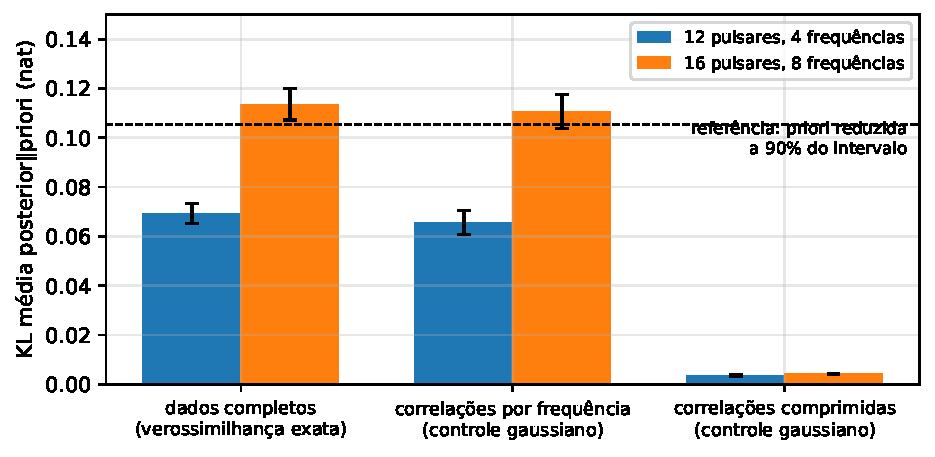
\includegraphics[width=.9\textwidth]{../figuras/informacao.pdf}
 \caption{Informação média sobre a massa, $D_{\rm KL}$ entre posterior
 e priori, em 500 realizações da campanha tensorial II, com erro
 Monte Carlo da média. A linha tracejada indica a informação de uma
 posterior que apenas exclui 10\% do intervalo a priori.}
 \label{fig:sim-informacao}
\end{figure}

Três lições decorrem desse resultado.

\paragraph{A compressão examinada destrói quase toda a informação
sobre a massa.} A compressão testada é uma média fixa, não otimizada,
dos estimadores sobre os canais. A perda era esperada pela
Eq.~\eqref{eq:pta-fraca}. A
distorção dispersiva decai como $1/k^2$, e a média sobre os canais dilui
o canal mais baixo, onde está quase toda a informação, com canais que
quase não dependem da massa. A análise local de Fisher na campanha
escalar confirma esse padrão com seis parâmetros. Algumas combinações
de parâmetros retêm 60--70\% da informação após a compressão, enquanto
a combinação mais afetada retém menos de 1\%. O resultado não se
estende automaticamente a outras compressões. Existem esquemas
construídos para preservar a informação sobre parâmetros escolhidos,
como a compressão pelo escore \autocite{alsing2018compression} e as
compressões de dados propostas para PTAs \autocite{vanhaasteren2013}.
Sua adequação à massa do gráviton não foi testada aqui.

\paragraph{Diferenças pequenas não validam uma aproximação quando os
dados informam pouco.} Na campanha tensorial II, as posteriores obtidas com a resposta
avaliada em $f_{\rm ref}=1/T$ (Eq.~\ref{eq:pta-fref}) foram comparadas
com as da resposta exata, sobre as mesmas correlações comprimidas. Em
50 realizações com ruído conhecido, os deslocamentos do limite superior
de 95\% de $u$ foram todos menores que $0{,}01$, e as médias ficaram
entre $-0{,}0044$ e $0{,}0041$. Esse resultado não basta para validar a
aproximação. Uma explicação plausível é a pouca informação: se as
correlações comprimidas quase não informam sobre a massa, as posteriores
das duas respostas ficam ambas próximas da priori e, por isso, próximas
entre si. Essa explicação é uma hipótese compatível com os resultados,
não uma relação causal demonstrada; testá-la exigiria repetir a
comparação em regimes com mais informação. Dois fatos pesam a favor dela.
Primeiro, as mesmas aproximações mudam apreciavelmente a distribuição
prevista dos dados perto do limiar quando o sinal é intenso
(Seção~\ref{sec:pta-informacao}). Segundo, a informação aparente não é
um indicador confiável quando o modelo está errado. Com as correlações
por frequência e a aproximação normal, a KL média foi de $0{,}099$ e
$0{,}146$~nat nas duas redes, \emph{maior} que a dos dados completos com a
verossimilhança exata ($0{,}069$ e $0{,}114$~nat). Uma análise incorreta
pode, portanto, exibir informação que os dados não contêm. Quando a
nuisance foi marginalizada, a comparação ficou inconclusiva na mesma
escala.

\paragraph{Limites superiores podem ser só a priori.} Se os dados não
informam nada, com verossimilhança constante e priori uniforme em
$u\in[0,1]$, a posterior é a própria priori. O limite de 95\% é então
$u=0{,}95$, isto é,
\begin{equation}
 m_gc^2\leq0{,}95\,\frac{h}{T},
 \label{eq:sim-priori}
\end{equation}
com $D_{\rm KL}=0$. Esse limite tem a escala natural $h/T$ de qualquer
limite obtido pelo suporte cinemático (Seção~\ref{sec:pta-informacao}).
A observação é elementar, mas tem consequência prática. Um limite de
massa próximo de $h/T$ deve vir acompanhado da informação efetivamente
ganha, por exemplo $D_{\rm KL}$ da marginal da massa, e da sensibilidade
à escolha da priori, para que se saiba quanto vem dos dados. Nas
simulações tensoriais, a calibração da massa foi satisfatória em todos
os métodos (coberturas de 455 a 460 em 500 no intervalo central de
90\%). Com posteriores tão próximas da priori, essa calibração é quase
automática e não atesta a qualidade da análise.

\section{A aproximação normal para as correlações}

As campanhas com parâmetros de ruído livres ou com o modo escalar
permitem testar a aproximação normal dos estimadores quadráticos, pois
nelas os dados contêm informação apreciável sobre algum parâmetro. A
Tabela~\ref{tab:sim-cobertura} mostra a cobertura de intervalos centrais
de 90\%, que deveria ser de cerca de 450 em 500.

\begin{table}[htbp]
\centering
\caption{Cobertura de intervalos centrais de 90\% em 500 realizações
(esperado: $\approx450$, com desvio padrão binomial $\approx7$).}
\label{tab:sim-cobertura}
\small
\begin{tabular}{lccc}
\toprule
Análise & Fator de ruído branco & $u$ & $\varepsilon$\\
 & (tensorial I) & (escalar) & (escalar)\\
\midrule
Dados completos, verossimilhança exata & 446 & 444 & 454\\
Correlações por frequência, aproximação normal & 313 & 365 & 436\\
Correlações comprimidas, aproximação normal & 412 & 422 & 451\\
Correlações por frequência, controle gaussiano & 449 & 452 & 449\\
Correlações comprimidas, controle gaussiano & 457 & 447 & 451\\
\bottomrule
\end{tabular}
\end{table}

Os controles gaussianos têm cobertura correta; portanto, a falha não
vem da redução dos dados nem de erro numérico. Ela vem de tratar como
normal um estimador que não é normal. A subcobertura é maior nas
correlações por frequência, em que cada estimador é uma soma de poucos
termos quadráticos e a assimetria é maior. A média sobre canais
aproxima a distribuição da normal e reduz o problema, sem eliminá-lo.
Testes de calibração baseada em simulação (SBC) \autocite{talts2018}
rejeitaram a uniformidade das aproximações normais em várias
estatísticas. Nenhuma rejeição ocorreu nas análises corretamente
especificadas.

\section{Falsas detecções de polarização escalar}

A consequência mais relevante para buscas de polarizações adicionais
aparece na campanha escalar. Em 500 simulações \emph{sem} modo escalar
($\varepsilon=0$), declarou-se detecção de helicidade zero quando o
fator de Bayes entre os modelos com e sem escalar excedeu 10. A
Figura~\ref{fig:sim-fp} mostra as taxas de declaração.

\begin{figure}[htbp]
 \centering
 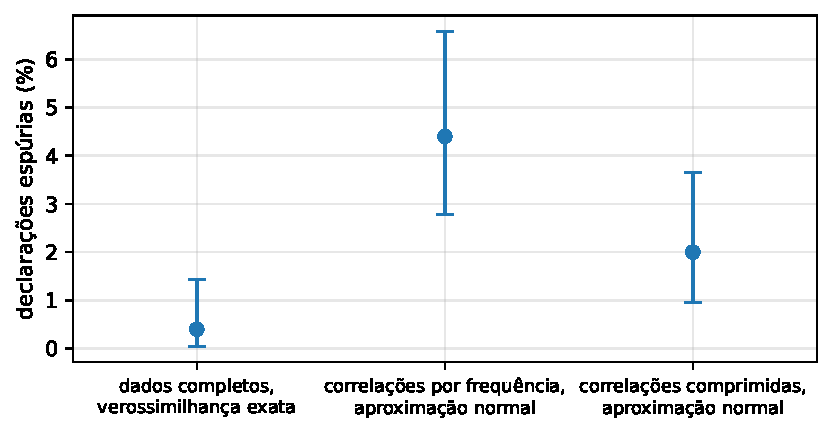
\includegraphics[width=.8\textwidth]{../figuras/falsos_positivos.pdf}
 \caption{Taxa de declarações espúrias de modo escalar
 ($\mathrm{BF}>10$) em 500 injeções puramente tensoriais, com
 intervalos de Clopper--Pearson de 95\%.}
 \label{fig:sim-fp}
\end{figure}

Com a verossimilhança exata, houve 2 declarações em 500 (0,4\%). Com a
aproximação normal para as correlações por frequência, 22 em 500
(4,4\%): a taxa de falsas detecções aumenta cerca de dez vezes. Com as
correlações comprimidas, houve 10 em 500 (2,0\%). Os controles gaussianos
tiveram 2 e 1 declarações. Novamente, o problema está na forma da
verossimilhança, não na redução dos dados.

A campanha também mostra o outro lado: o poder de detecção de uma rede
pequena é baixo. Com massa $u=0{,}2$ e potência escalar igual à metade
da tensorial ($\varepsilon=0{,}5$), a análise exata declarou o modo
escalar em apenas 3 de 32 realizações. Perto do limiar ($u=0{,}995$),
não houve nenhuma declaração, como esperado pela degenerescência da
Seção~\ref{sec:pta-degenerescencia}. Nesse mesmo regime, a massa foi sistematicamente
subestimada: as medianas posteriores ficaram em torno de $0{,}7$--$0{,}8$
e a cobertura central foi de 0 a 3 em 32. Isso é um efeito da fronteira
da priori combinado com pouca informação, não uma falha numérica.

Em conjunto, os dois resultados indicam um risco para buscas de
polarizações. Com dados pouco informativos, a aproximação normal usual
produz mais ``detecções'' espúrias do que o poder real de detecção
justificaria. A verossimilhança dos estimadores deve ser testada no
regime de sinal e ruído relevante antes de interpretar uma preferência
por polarizações adicionais \autocite{franciolini2025}.

\section{Dos coeficientes periódicos aos tempos de chegada}
\label{sec:sim-timing}

O modelo \eqref{eq:sim-modelo} supõe canais de frequência independentes.
Em dados reais, o ajuste do modelo de temporização remove polinômios em
$t$ (fase, frequência e derivada de rotação) e termos anuais
(astrometria). Um experimento auxiliar com um pulsar, 256 observações em
4,5 anos e ruído vermelho de índice $13/3$ quantificou esse efeito.
Mesmo com amostragem regular, o ajuste introduz correlações entre
canais e uma pseudocovariância não nula, ausentes no modelo periódico.
Ignorá-las resultou numa divergência de 11 nat entre a distribuição
verdadeira dos oito primeiros coeficientes e a aproximação por canais
independentes. As previsões analíticas foram confirmadas com 20.000
realizações. Esse efeito é conhecido na análise de PTAs
\autocite{vanhaasteren2013}. O experimento apenas mostra que ele é
grande justamente nos canais mais baixos, que são os que contêm a
informação sobre a massa.

\section{Limitações e o que seria necessário}
\label{sec:sim-limitacoes}

As campanhas deste capítulo têm limitações que devem ser explicitadas.
\begin{itemize}
 \item \textbf{Regime pouco informativo.} As redes simuladas são pequenas
 e, na campanha tensorial II, o sinal é fraco e a duração é curta. Esse
 foi o principal defeito do desenho: as comparações entre análises foram
 feitas onde quase não há informação sobre a massa, e por isso muitas
 delas não discriminam.
 \item \textbf{Ruído conhecido.} Nas campanhas II e escalar, a amplitude
 e o espectro do sinal e do ruído foram fixados. Com esses parâmetros
 livres, a informação sobre a massa seria ainda menor.
 \item \textbf{Modelo periódico.} Sem ajuste de temporização nem
 amostragem irregular (Seção~\ref{sec:sim-timing}).
 \item \textbf{Distâncias conhecidas.} Perto do limiar, as correlações
 dependem das distâncias (Capítulo~\ref{cap:pta}), que em dados reais são
 incertas.
\end{itemize}

O passo seguinte natural é uma previsão de sensibilidade para uma rede
realista. Ela deveria usar dezenas de pulsares, 15 a 20 anos de dados e
a amplitude medida, e marginalizar o ruído e as distâncias. Deveria
também perguntar diretamente qual a menor massa e qual a menor fração
escalar que podem ser distinguidas da RG. As ferramentas desenvolvidas
já comportam esse estudo: resposta com termos dos pulsares, setor
escalar vinculado e controle do erro numérico. As lições metodológicas
deste capítulo valem para os cenários testados e devem ser reavaliadas
nesse novo regime. Elas indicam três cuidados: testar a verossimilhança
dos estimadores no regime de interesse, verificar quanta informação
sobre a massa uma eventual compressão preserva e reportar a informação
ganha junto com os limites.
